\documentclass[tikz]{standalone}

\colorlet{FilledSurface}{blue!20}
\colorlet{FilledSurfaceGroupOne}{blue!20}
\colorlet{FilledSurfaceGroupTwo}{red!20}
\colorlet{FilledSurfaceGroupThree}{green!20}
\colorlet{FilledSurfaceGroupFour}{magenta!20}
\colorlet{FormulaBackground}{green!10}
\colorlet{FormulaFrame}{green}


\usetikzlibrary{calc, intersections, decorations.markings, angles}

\tikzset{
    mark rect/.style={
        decoration={markings, mark=at position 0.5 with {
            \draw[fill=white] (-6pt,-2pt) rectangle (6pt,2pt);
        }}, postaction={decorate}
    },
    mark one circle/.style={
        decoration={markings, mark=at position 0.5 with {
                \draw[fill=white] (0,0) circle (2pt);
        }}, postaction={decorate}
    },
}

\begin{document}
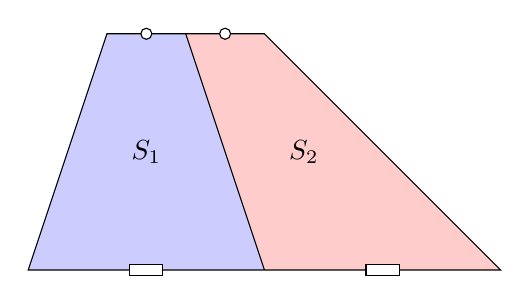
\begin{tikzpicture}

\coordinate (A) at (0, 0);
\coordinate (B) at (1, 3);
\coordinate (C) at (3, 3);
\coordinate (D) at (6, 0);

\coordinate (M) at ($(B)!0.5!(C)$);
\coordinate (N) at ($(A)!0.5!(D)$);

% Colorear superficies
\fill[FilledSurfaceGroupOne] (A) -- (B) -- (M) -- (N);
\fill[FilledSurfaceGroupTwo] (M) -- (C) -- (D) -- (N);

% Dibujamos los segmentos, luego de colorear las superficies para
% evitar que las superficies cubran a los segmentos.
\draw (A) -- (B) -- (C) -- (D) -- cycle;
\draw (M) -- (N);

\path[mark one circle] (B) -- (M);
\path[mark one circle] (C) -- (M);
\path[mark rect] (A) -- (N);
\path[mark rect] (D) -- (N);

\node at (barycentric cs:A=1,B=1,M=1,N=1) {$S_1$};
\node at (barycentric cs:M=1,C=1,D=1,N=1) {$S_2$};
\end{tikzpicture}
\end{document}
